\documentclass{article}

\usepackage{graphicx}
\usepackage[left=2cm, right=2cm, top=2cm]{geometry}

\usepackage{xcolor}
\newcommand\fixlater[1]{\textcolor{red}{#1}}

\begin{document}

% The following part of this document will be placed in the Methods section

The next test determines how well the three solvers perform for decreasing
values of the mass ratio. This test is done for the binary lens. The three
solvers are: the numpy root solver, the method by Skowron and Gould 2012, and
Numerical Recipes zroots method. This test uses the same methodology of
plotting the number of images and the magnification on a grid of points in
the source plane, and comparing the performance of each solver. All
caluclations were done using the form of the polynomial derived in the
planet frame, for a constant value of $s$. \textbf{Figure 1} shows the
plot of the number of images, and \textbf{Figure 2} shows the plot of
the magnification.

\begin{figure}
	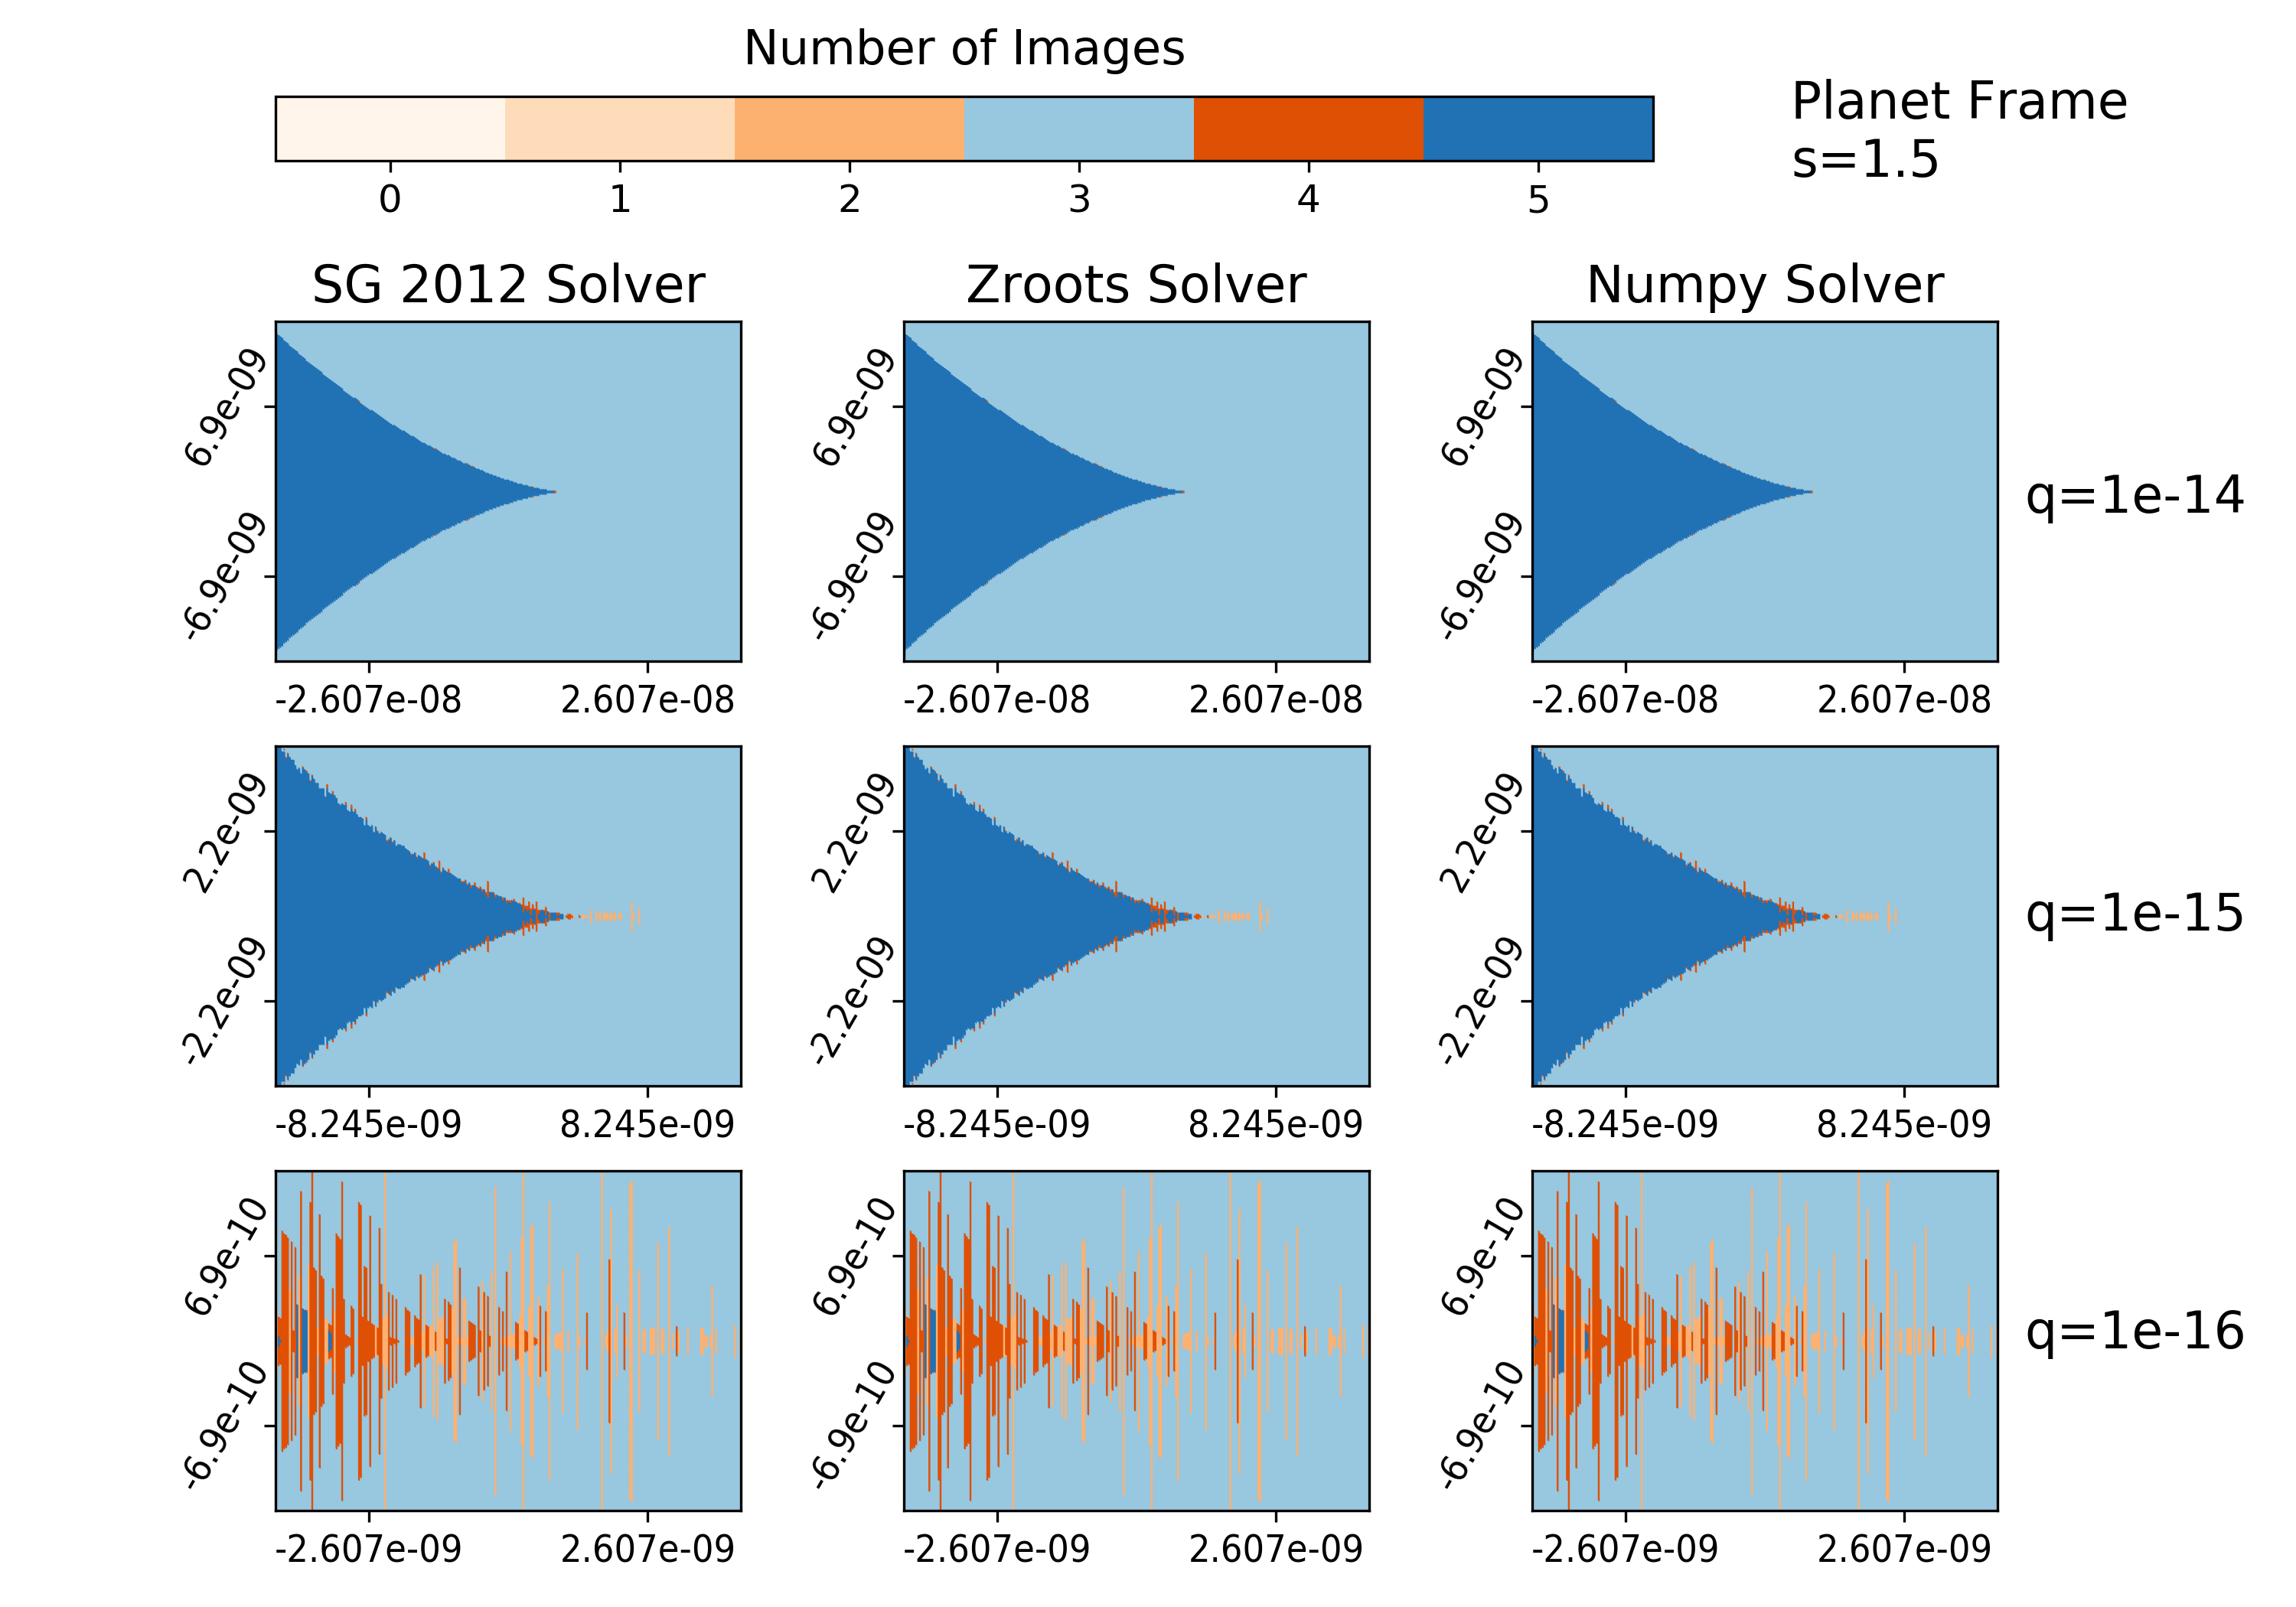
\includegraphics[width=0.9\textwidth]{../Tables/images_plan_solver_0.png}
	\caption{The number of images versus the position for each root solver
	in the planet frame. The rows coorespond to different values of the
	mass ratio, $q$. All solvers perform the calculations equally well in
	each row for the planet frame.}
\end{figure}

\begin{figure}
	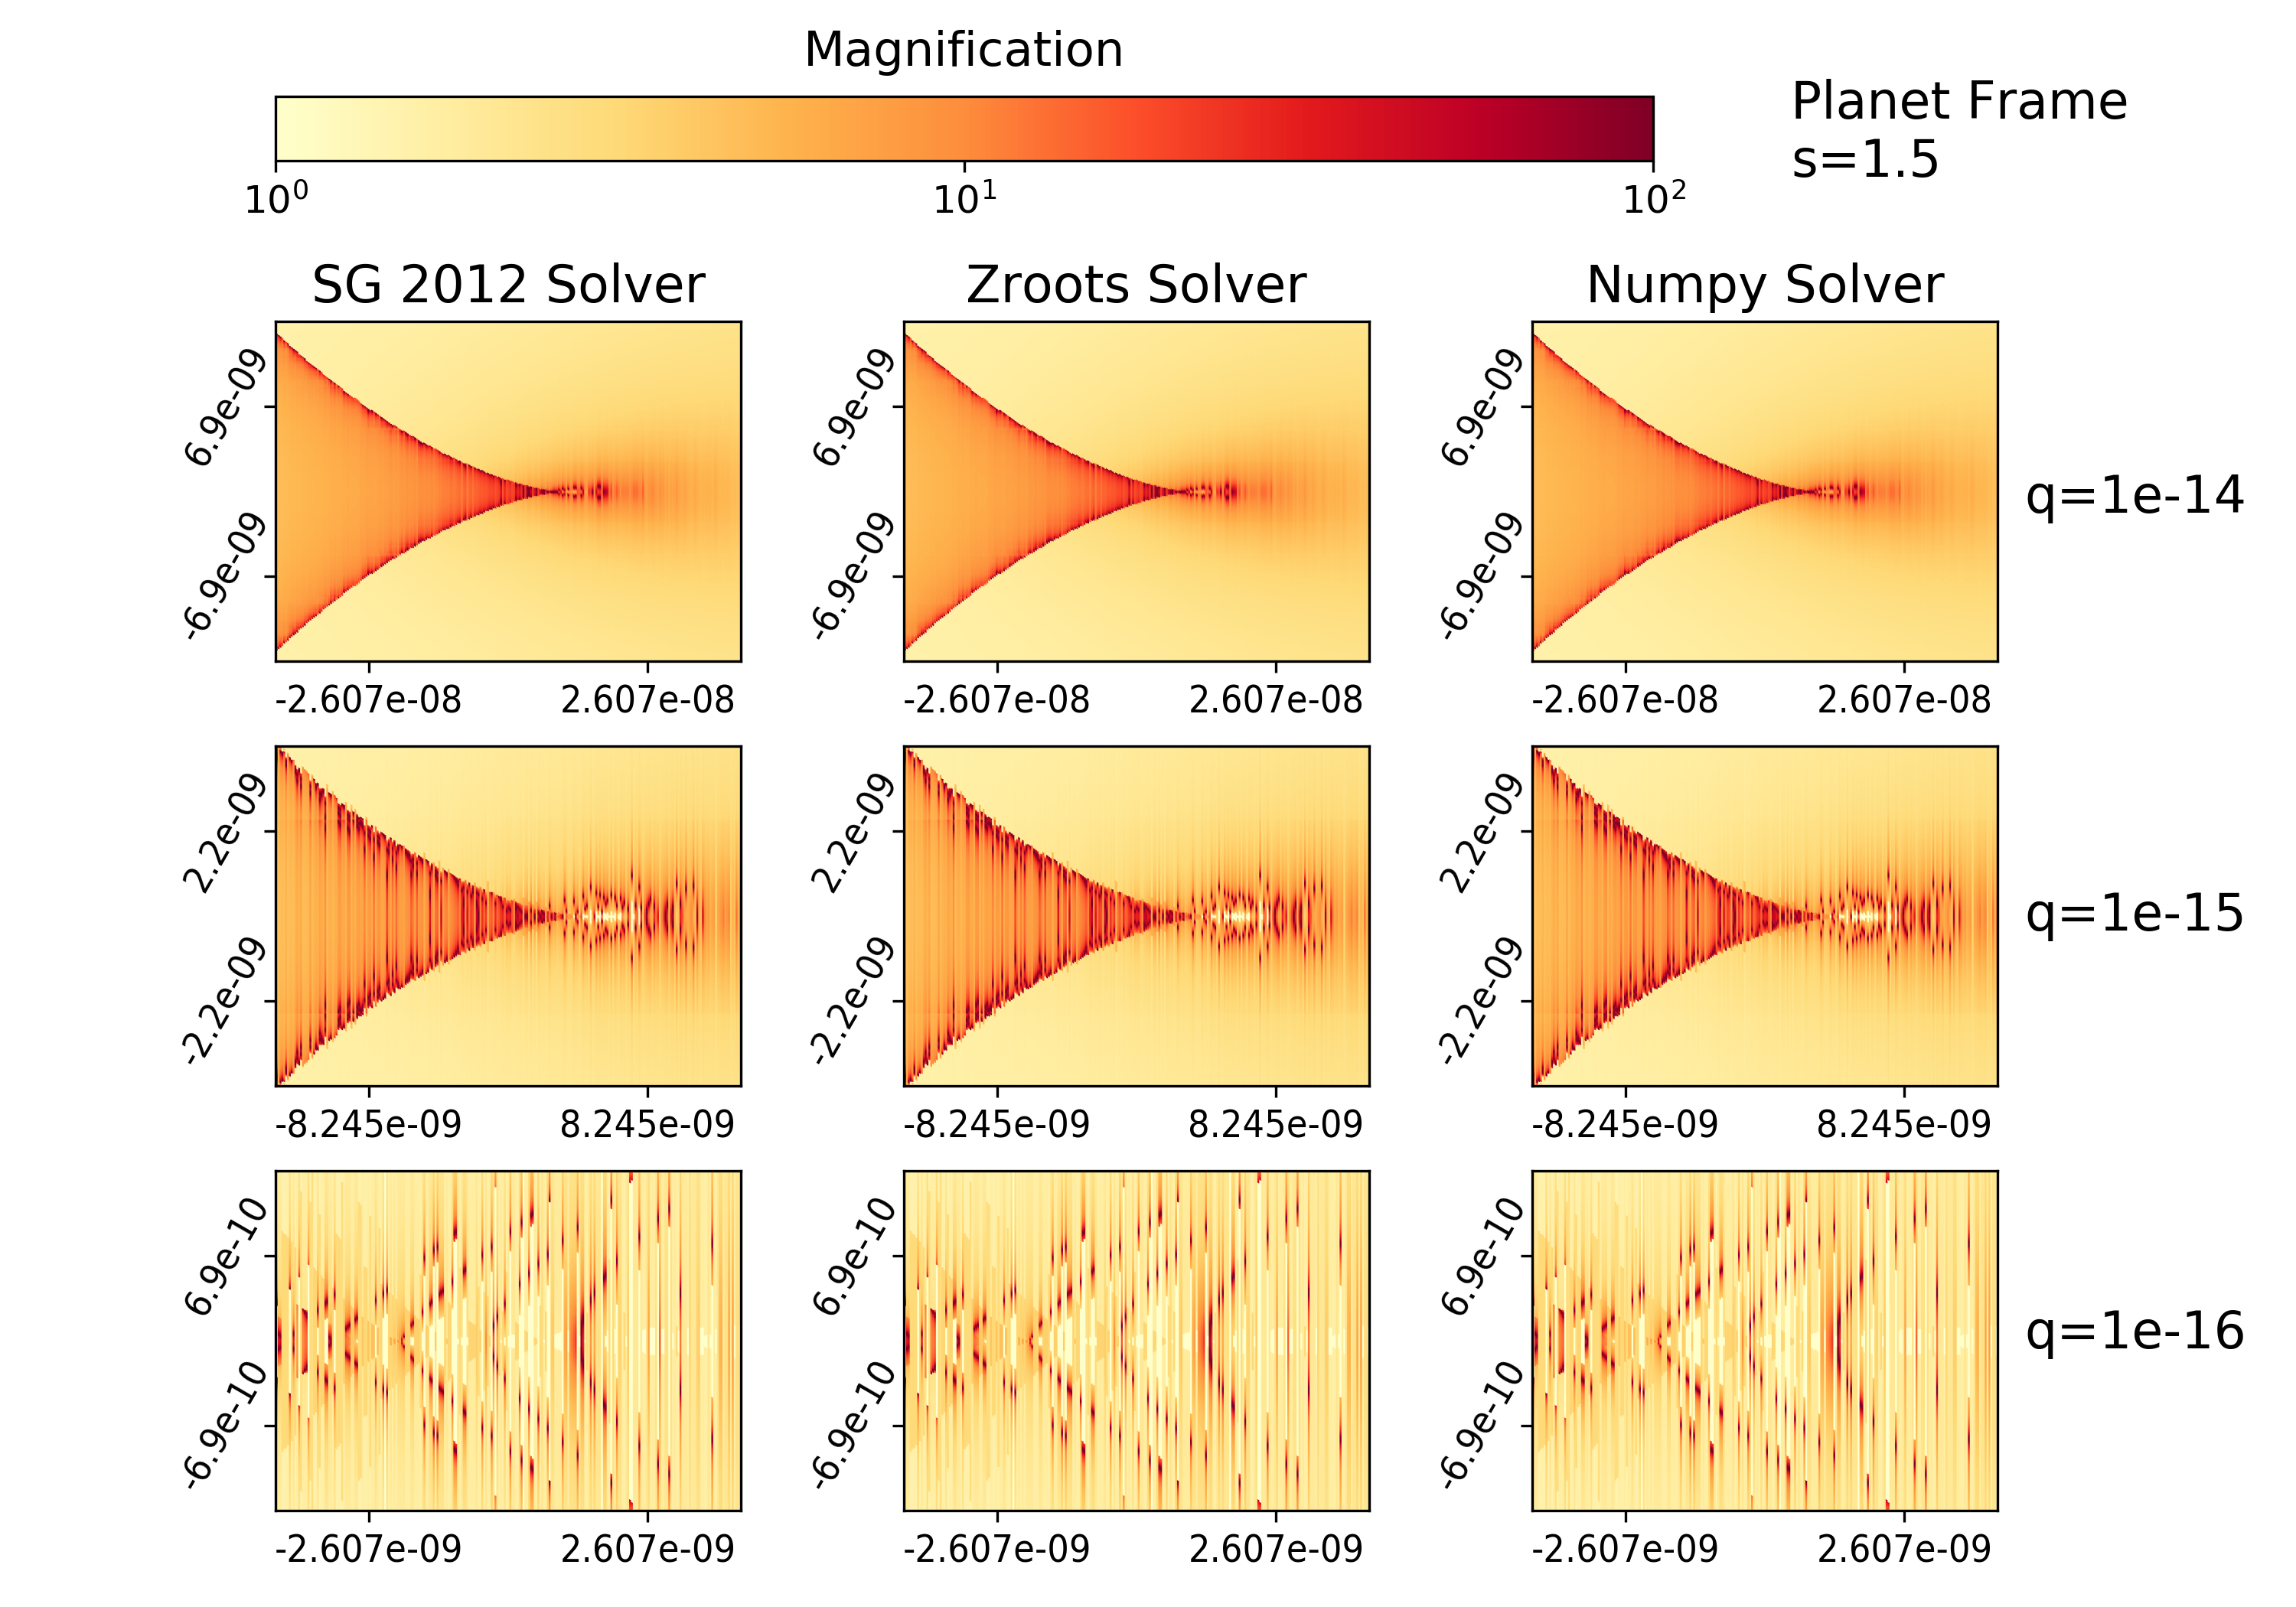
\includegraphics[width=0.9\textwidth]{../Tables/magn_plan_solver_0.png}
	\caption{Same as \textbf{Figure 1}, except with magnification. Again,
	all solvers perform the calculations equally well in each row for the
	planet frame.}
\end{figure}

% The following part of this document will be placed in the Results/Analysis
% section

This simulation does not suggest any deviation in how well the solvers
perform in the planet frame. They all make the same number of errors 
for a given mass ratio, $q$, as $q$ approaches its lower limits. Regardless
of the fact the solvers performed with the same accuracy, there is evidence
in (\fixlater{insert citation}) that the Skowron and Gould 2012 method performs
the fastest.

\end{document}
